\section{Back-test results}

The implementation of back-test results is based on running the portfolio revision model for each month until the last portfolio revision at 2014-06-18.
The portfolio revision model is performed for each month, where $x^\up{old}_{i}$ is updated every run, with the previous portfolio updated with the historical month return of the current month.
I.e. $x_i^\up{old} \leftarrow (1 + HMR_{i,m}) * x_i$.

\begin{figure}[tpb]
\centering
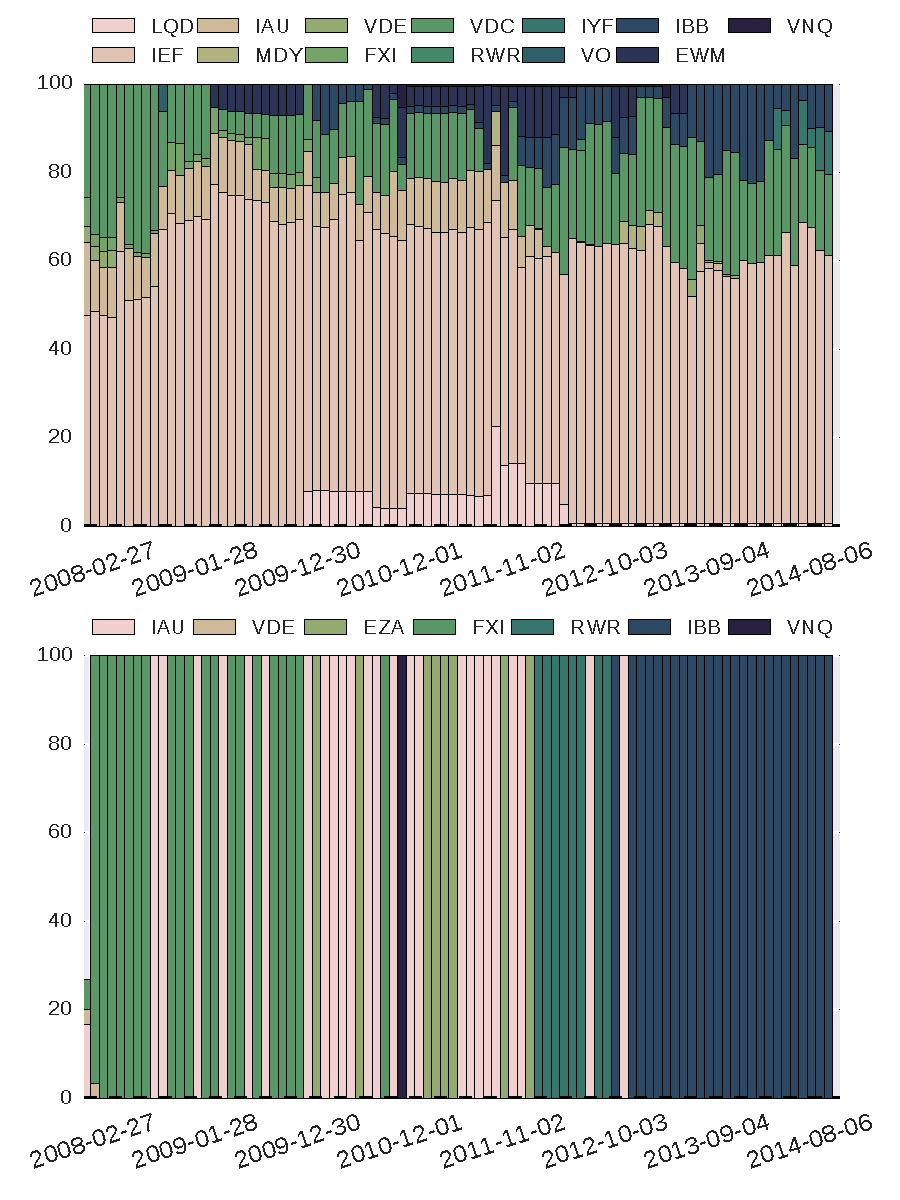
\includegraphics{../pic/trading_portfolio.pdf}
\caption{Portfolios found by the risk-averse (top) and risk-neutral (bottom) trading strategies.}
\label{fig:tradingportfolios}
\end{figure}

The optimal portfolio mix for each period considering all its revision for both risk averse and risk neutral strategies are illustrated in Figure~\ref{fig:tradingportfolios}.
The risk averse strategy always obtain a mixed portfolio in order to minimize the risk of bad return.
One can verify that the IAU assets is in general the base of the portfolio mix for risk averse strategy.
Looking at the risk neutral strategy, on the other hand, it tries to bank on the single asset with the largest expected return.
At early times, the FXI asset has high participation, since that ETF has an upward tendency until the crash. After the crash, IAU has a very good upward tendency.
At this point IBB start slowly a upward tendency, which is more steeper in later periods.
In this way and based on the behaviour of the ETFs in Figure~\ref{fig:prices_selected}, the portfolio revision obtained for both perspectives is as expected.

\begin{figure}[tpb]
\centering
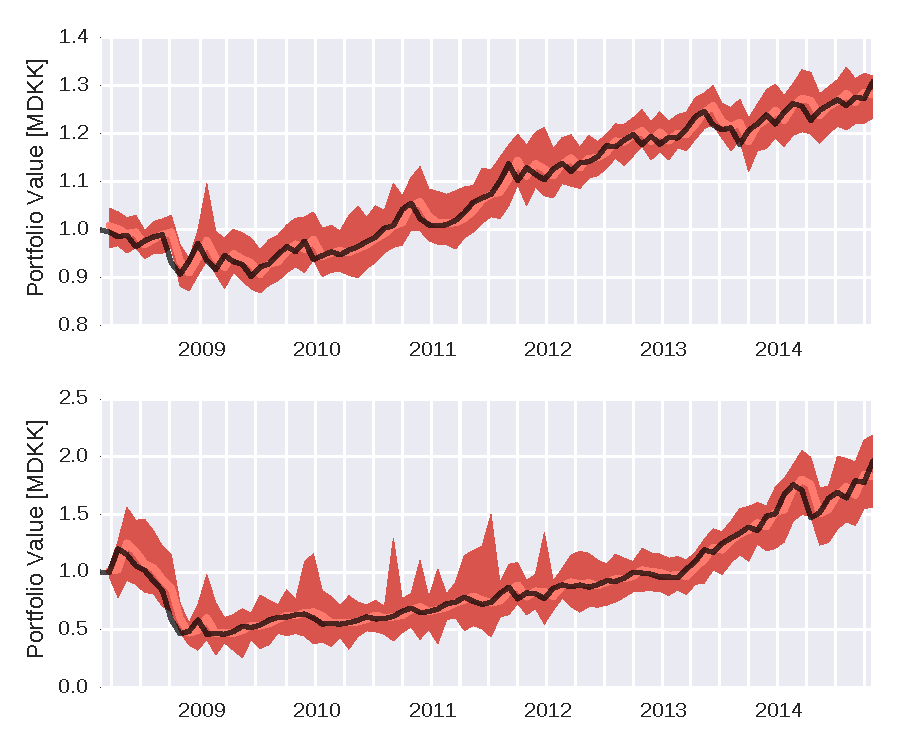
\includegraphics{../pic/trading_forecasted_value.pdf}
\caption{Nominal values of portfolios over time (Black line) versus forecasted mean value (light red). The shaded region indicates the maximum and minimum forecasted values of the ensembles. The risk avers (top) and risk neutral (bottom) strategies for portfolio valueare considered.}
\label{fig:tradingforecastedvalues}
\end{figure}

The historical values of the portfolios found is compared to that forecasted by the scenarios of the previous trading period in Figure~\ref{fig:tradingforecastedvalues}.
The forecasted values always seem to trail the actual values by 1 month.
This is explained as the result of the forecast essentially being a persistence forecast due to the small average return provided.

Looking at the spread the scenarios reveal that only in a few cases around mid-late-2008 do the returns fall outside the interval predicted by the forecast, indicating that the scenarios are able to capture the risk in the market, despite missing the movement of the portfolio mean.

\begin{figure}[tpb]
\centering
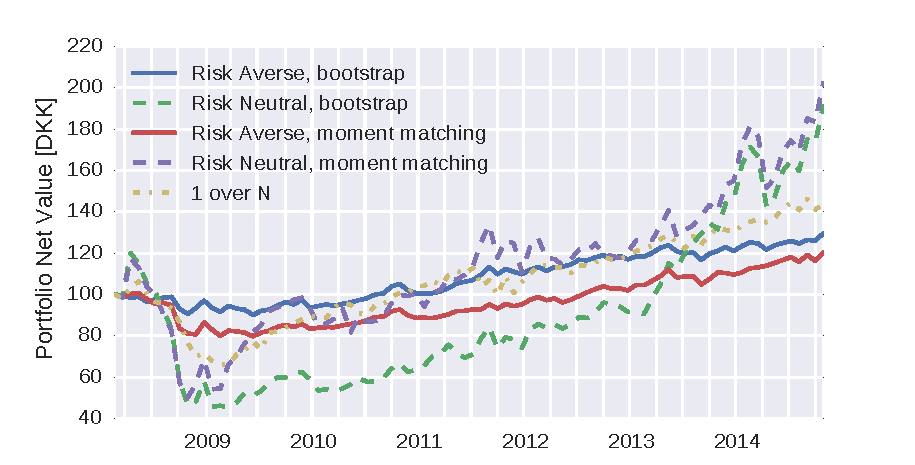
\includegraphics{../pic/trading_portfolio_value.pdf}
\caption{Net values of portfolios over time. (Net value = nominal value minus cumulative trading costs)}
\label{fig:tradingportfoliovalues}
\end{figure}


% TODO: REWRITE

The portfolio value over the time for each of the strategies is presented in Figure~\ref{fig:tradingportfoliovalues}.
One can see that different strategies has different average behaviours, as well as the worst and best case of the scenarios.
The risk neutral strategy is the strategy that achieves higher return in the end of the period of investment. 
However, it does not mean that is the best strategy among all periods.
On average, the ideal strategy throughout the time is the use of both strategies to maximize the expected return.
In the early six months is advised the use of risk neutral strategy.
Than risk averse should be used until the early months of 2013.
In the remaining months, risk neutral ensures more return to the investor.

Regarding the results of portfolio revision model considering the scenario generation of moment matching, we conclude that the patterns of the results are very similar.

To compare the strategies with a simple trading scheme, the $1/N$ strategy is used; on the first trading day we invest an equal amount into each asset, and then leave the assets be for the entire trading period.
In order to compare a 1/N strategy with the strategy results of risk averse and risk neutral is presented the Figure~\ref{fig:tradingportfoliovalues}.
Furthermore, is considered the results of each strategy (risk averse and risk neutral) for each scenario generation method (bootstrap and moment matching).

One can see that the risk averse strategy from the bootstrap method present on average higher portfolio value than the same strategy but based on moment matching method.
On the other hand, risk neutral strategy from moment matching strategy presents on average higher portfolio values than the strategy based on bootstrap method.
Regarding to the 1/N strategy, one can identify that is a strategy that returns a stable portfolio value throughout the periods.
However, is a strategy that presents results between the two extreme strategies (risk averse and risk neutral).
In the end, is expected a higher return value on risk averse strategy, and the lower return value on risk neutral strategy.

% Until here

\begin{table}[tpb]
\caption{Comparison of trading strategies}\label{tbl:strategytabel}
\centering
\begin{tabular}{lrrrl}
\toprule
{} & Final Nominal &  Trading &  Final Net & Annualized \\
{} & Value & Costs & Profit & Return \\
\midrule
Risk Averse, bootstrap        &              1259714 &          10810 &            248904 &             3.6 \% \\
Risk Neutral, bootstrap       &              1639882 &          43283 &            596599 &             7.7 \% \\
Risk Averse, moment matching  &              1172530 &           5797 &            166733 &             2.5 \% \\
Risk Neutral, moment matching &              1701345 &           8787 &            692558 &             8.7 \% \\
1 over N                      &              1462676 &              0 &            462676 &             6.2 \% \\
\bottomrule
\end{tabular}

\end{table}


A comparison between the final numbers of the trading strategies is shown in Table~\ref{tbl:strategytabel}.
Four things are noteworthy here:

Firstly, the highest return for the risk averse strategies is found by the boostrap scenarios rather than the moment matching ones, whereas they perform oppositely for the risk neutral strategy.
This is reasonable, as the risk averse strategy is sensitive to correlations in the data, which are destroyed by the moment matching scenarios, while the risk-neutral strategy needs an accurate representation of the mean, which is captured more closely by the moment matching scenarios.

Secondly, the trading costs are much higher for the bootstrap scenarios than for the moment matching scenarios.
This may be understood as the bootstrap scenarios can change quite a lot over time, while the moment matching scenarios will tend to jump around less in between time steps.

Thirdly, the trading costs are higher for the risk neutral strategy than for the risk averse strategy. This is due to the risk neutral strategy constantly throwing away the entire portfolio as shown on Figure~\ref{fig:tradingportfolios}.

Fourthly, the 1 over N strategy manages to outperform both risk averse strategies, and would have outperformed the risk neutral strategies as well if the market hadn't experienced a steady upswing in 2013 and 2014.

As a closing remark, taking the old advice to just bet on gold, and invest everything in IAU, cashing out in 2012 would have given an annualized return across the period of $9.4 \%$. If this money had then been reinvested in IBB, the annualized return would have been $\sim 27 \%$.
In other words, clairvoyance outperforms any mortal strategy.